\section{Bitcoin}
Bitcoin was invented in 2008 by Satoshi Nakamoto~\cite{bitcoin} as a peer-to-peer version of electronic cash, allowing online payments to be sent directly between parties without the need of a intermediary.

Bitcoin is pseudonymous: the identity of each user is only their \emph{address}, which corresponds to an ECDSA public key. This address can be used to receive money from other users. Each user can spend money only if they have their corresponding private key. A set of ECDSA keypairs comprises a \emph{wallet}. A user can have multiple addresses.

\begin{figure}
  \centering
  \code{1A1zP1eP5QGefi2DMPTfTL5SLmv7DivfNa}
  \caption{A Bitcoin address}
  \label{fig:address-example}
\end{figure}

Transfer of value in Bitcoin happens with transactions. A transaction has inputs and outputs. An output is where the value creation happens for the receiver. An output can be later redeemed by using its designated receiver's private key and turned into an input to be used for another transaction.

\subsection{Scripts}
Bitcoin offers much more than just moving currency around. It allows us to actually move currency conditionally, where the condition can be expressed as a \emph{Bitcoin script}. Bitcoin script is a stack-based language. An example of a Bitcoin script can be seen on Figure~\ref{fig:bitcoin-script}.

\begin{figure}
  \centering
  {
    \tt
    OP\_HASH256 \\
    6fe28c0ab6f1b372c1a6a246ae63f74f931e8365e15a089c68d6190000000000 \\
    OP\_EQUAL
  }
  \caption{A Bitcoin script}
  \label{fig:bitcoin-script}
\end{figure}

This is an interesting script because it introduces two kinds of operations. First is commands prefixed with \code{OP\_} (called \emph{opcodes}): these perform operations on values (usually the top 1 or 2) on the stack and push the result to the stack. Specifically, \code{OP\_HASH256} calculates the SHA256 hash of the value on the top of the stack (and pushes the result on the stack). \code{OP\_EQUALS} compares the top 2 values on the stack and pushes 1 or 0 if they are indeed equal or not accordingly. Values like \code{6fe...} in hex with no \code{OP\_} prefix are simply pushed to the stack.

So what does this script do? It checks if the value on the stack is the preimage of the given hash. If we do push the correct preimage in the stack before running the script, the result is going to be 1, letting us know that the evaluation was successful.

Such a script express our predicate, and is called a \textsf{pubKeyScript}. However the predicate must run on something. In our example above we assumed the preimage was on the stack before the stack ran, and this is how we parameterized our predicate. The way this is done in Bitcoin is running another script before the predicate called \textsf{scriptSig}, to essentially pass the parameters to our predicate. We'll see shortly how these can be leveraged to actually transfer funds.

It's important to note that there's a third type of opcodes which can fail the script preemptively. These opcodes are usually in the form of \code{OP\_...VERIFY}. An example is \code{OP\_EQUALVERIFY} which fails the script if the top 2 values of the stack are not equal, and is otherwise a no-op.

Next we'll look at a couple of interesting classes of scripts.

\subsubsection{Anyone-can-spend}
It's easy to make the predicate true for everyone. We can make \textsf{pubKeyScript} be \code{OP\_TRUE} (which adds the true value to the stack) and \textsf{scriptSig} be empty.

\subsubsection{P2PKH}
This is the standard script for conventional fund transfer in Bitcoin. Let's say we want to make sure only Bob can satisfy this script. The \textsf{pubKeyScript} is the following: \code{OP\_DUP OP\_HASH160 <Bob's address> OP\_EQUALVERIFY OP\_CHECKSIG}.

The \textsf{scriptSig} is then typically \code{<Bob's signature> <Bob's public key>}. Values in \code{<>} are placeholders for actual values, they're not valid script commands. These have to be replaced with concrete values before the above scripts can be valid.

Bob's signature will be on the hash of the transaction (which we'll explore shortly) containing the output. The script will then duplicate his public key, check that it matches the one on the \text{pubKeyScript}, and if it does check that he has provided a valid signature with that public key. If all these checks pass the stack will end up with 1 on top and the execution will be valid, thus the predicate will be satisfied.

\subsubsection{OP\_RETURNs}
It frequently is desired to add arbitrary data to the blockchain (e.g. for timestamping). To do this, one can make the arbitrary data part of the \textsf{pubKeyScript}. There's a special opcode for such cases called \code{OP\_RETURN} which can be followed by a series of arbitrary data (in hexadecimal). \code{OP\_RETURN} fails the script preemptively so no \code{scriptSig} can satisfy it. We'll see how based on \code{OP\_RETURN}s we can greatly augment the functionality of Bitcoin later on.

\subsection{Outputs}
An \emph{output} is a tuple ({\sf value, pubKeyScript}). The \textsf{value} refers to an amount of Bitcoin in Satoshi (where $\sf 10^8 \, Satoshi = 1 \, Bitcoin$) and \textsf{pubKeyScript} is a script which needs to be run against some stack and return 1 in order for \textsf{value} to be transferable.

\subsection{Inputs}
An input is the way an output is redeemed. Specifically, it contains 3 things:
\begin{itemize}
  \item The hash of the transaction where the output of interest is contained.
  \item An index clarifying which output in the transaction this input is referring to.
  \item A signature (called \textsf{scriptSig}) used for the validation of the output script.
\end{itemize}

For the transaction to be valid, the script inside the specified output when run on a stack with the contents of \textsf{scriptSig} should return 1.

As a convention, when we talk about the value of an input we mean the value of the output it redeems.

\subsection{Transactions}
A \emph{transaction} is a collection of inputs and outputs. It uses the sum of the inputs values' as credit to debit each output accordingly. As it makes sense, a transaction is only valid as long as all its outputs and inputs are valid. It should also be clear that the value of the outputs should not exceed the value of the inputs, otherwise we would be creating value out of thin air with new transactions. Specifically this is expressed as $\sum_{\sf i \in inputs} {\sf i.value} \ge \sum_{\sf o \in outputs} {\sf o.value}$. This is sometimes called the \emph{Law of Conservation}.

In cases where $\sum_{\sf i \in inputs} {\sf i.value} > \sum_{\sf o \in outputs} {\sf o.value}$ we call
$$\sum_{\sf i \in inputs} {\sf i.value} - \sum_{\sf o \in outputs} {\sf o.value}$$
the \emph{transaction fee}. This is paid to the miner who successfully mines a block containing the transaction. This is one of the two ways Bitcoin uses to incentivize miners.

\begin{figure}
  \centering
  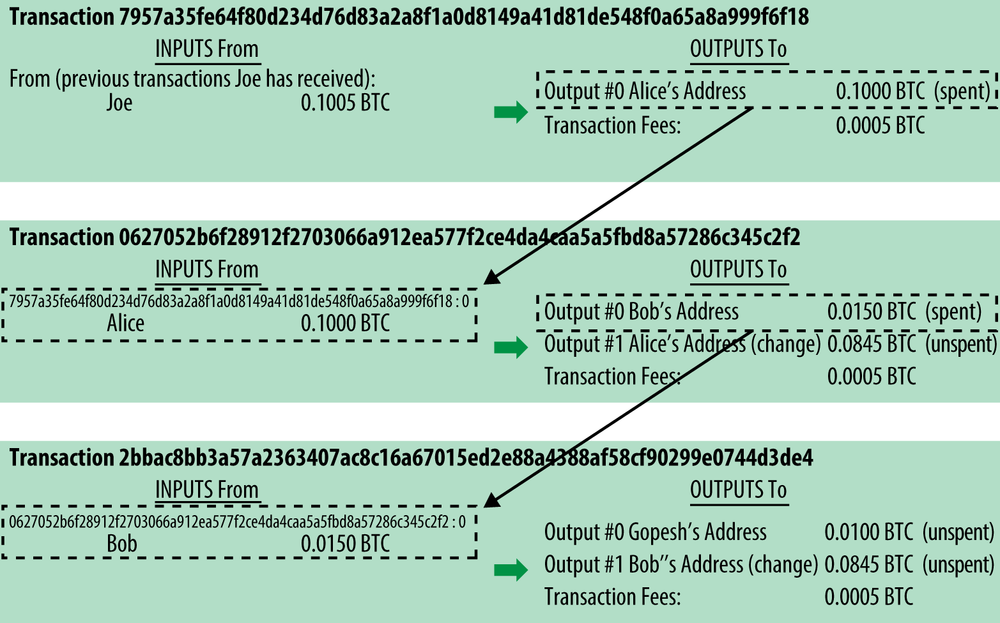
\includegraphics[width=0.9\columnwidth,keepaspectratio]{figures/transaction-internally.png}
  \caption{Transactions with their inputs and outputs.  Source:~\cite{mastering}}
  \label{fig:transaction-internally}
\end{figure}

\subsection{Blocks}
A block contains a list of transactions, the first of which is called the \emph{coinbase transaction} which is where value creation happens in Bitcoin. The miner crafts this transaction granting them some amount of Bitcoins and this transaction is going to be valid only if the block turns out valid. This doesn't mean that anyone can generate Bitcoin out of thin air: we'll see shortly how it actually comes at a cost with Proof-of-Work.

\begin{figure}
  \centering
  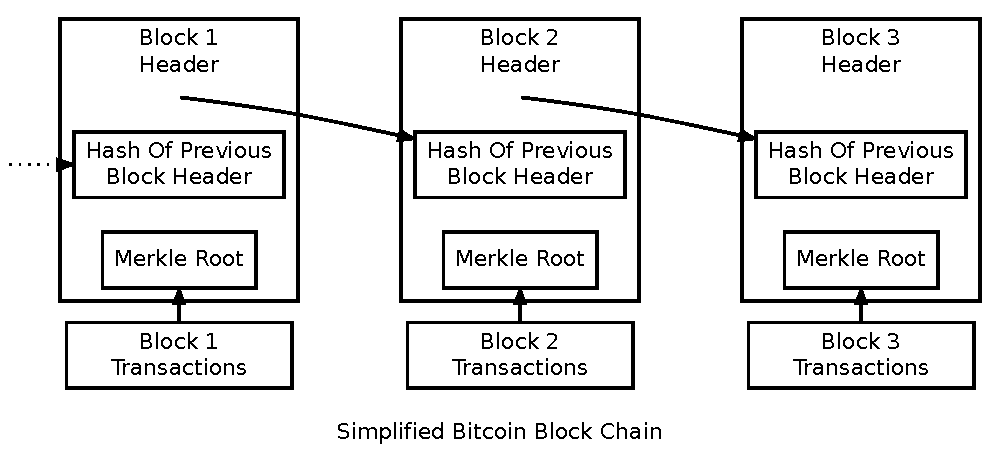
\includegraphics[width=0.9\columnwidth,keepaspectratio]{figures/block-structure.pdf}
  \caption{The block structure.  Source:~\cite{bitcoin}}
  \label{fig:block-structure}
\end{figure}

A block header contains mainly the hash of the previous block, a Merkle root hash to commit to a set of transactions, and a nonce. Blocks are always referenced by the hash of their block header.

\begin{figure}
  \centering
  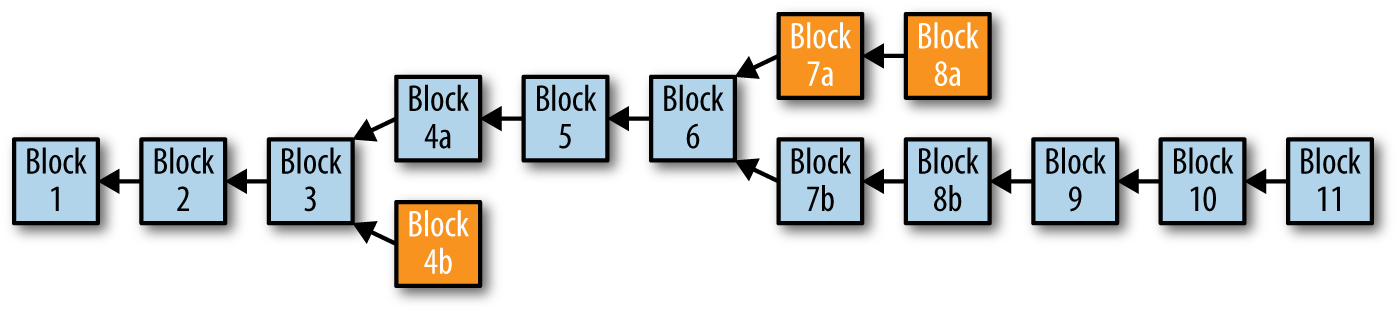
\includegraphics[width=0.9\columnwidth,keepaspectratio]{figures/blocks.png}
  \caption{A block chain. The orange blocks are orphans.  Source:~\cite{mastering}}
  \label{fig:blocks}
\end{figure}

Once a transaction has been included in a valid block it's called \emph{confirmed}.

It's possible that there are contending chains of blocks. We then say there is a \emph{fork} on the chain. On Figure~\ref{fig:blocks}, the chain has forked on blocks 3 and 6.

We call any valid blocks which are not part of our active chain \emph{orphans}. For example, on Figure~\ref{fig:blocks}, blocks 4b, 7a and 8a are orphans.

\subsection{Proof-of-Work}
The key to making Bitcoin decentralized is a technique called Proof-of-Work. Proof-of-Work was first invented in 1992 by Dwork et al.~\cite{dwork} as a measure of limiting email spam and denial-of-service attacks and later explored by Back~\cite{hashcash} as Hashcash.

We'll examine a simplified model of Hashcash in order to explore the idea. Suppose we want to send an email to someone. In order to prove we've done work, we include a header (like \code{X-Hashcash}), which (very simplistically) includes the receiver's email address, and a nonce.
\footnote{Hashcash headers actually contain 7 different fields which have been omitted here for simplicity. The simplified version explained here is not making the same security guarantees as Hashcash.}
The nonce is picked so that the hash of the header $H(email || nonce)$ has its 20 most significant bits be all 0. The only feasible way to find this is by brute-forcing the nonce. Once the sender has found the nonce it's included in the header and sent.

The receiver can then very easily check whether the header hashes to a valid value. If that's so, the email it contains belongs to the receiver and the header is not being reused, then the email can be considered not spam.

To reiterate, the idea is having a series of data to commit to and a hole for the nonce, which is brute-forced to satisfy a necessary predicate on the hash, specifically that its $n$ most significant bits are all zeroes. This is exactly how Bitcoin implements Proof-of-Work. Instead of the hole being on an email header the hole is on the block header. For a block to be valid, its header has to satisfy a predicate like the above.

Bitcoin introduces a couple of differences. $n$ varies according to the block generation rate. Specifically, to translate the previous predicate to Bitcoin terminology, the hash of each block header has to satisfy $H({\sf blockHeader}) \le T$ where $T$ is called the \emph{target}. As the target goes up, the probability of being below it goes up and generating a valid block is easier. Conversely, if the target goes down it's harder to generate a valid block. To express this, in Bitcoin $\frac{1}{T}$ is called the \emph{difficulty}.

To account for the block generation rate, which Bitcoin tries to keep to 1 block per 10 minutes, every 2016 blocks the target (and subsequently the difficulty) is adjusted accordingly. The target is calculated inside the Bitcoin software and is only as a function of the blocks previously seen (frequently called their \emph{view}), so as long as the Bitcoin nodes agree on the view they'll agree on the target and all consider the same set of incoming blocks as valid.

\subsection{\label{subsec:spv}Simplified Payment Verification}
The size of the blockchain has reached 185GB by September 2018, which makes it a very time consuming or even infeasible process to synchronise a full node. Fortunately, a solution was proposed in the original whitepaper ~\cite{bitcoin}, which allows the creation of so-called \textit{lite nodes}.  Lite nodes only know the headers of the entire blockchain, which are constant-size for each block (80 bytes). At the time of writing of this paper, the size of all block headers was $\sim$42MB. The lite node then asks the network for transactions concerning it (e.g.\ transactions concerning a specific public key). Full nodes of the network find such transactions and return them to the requester. For each transaction, the block header of the block it's included in is returned, along with a Merkle tree proof of inclusion which the lite node can then verify. This protocol is reliable as long as an adversary does not control the network of a lite node.

\subsection{Bitcoin Cash}
In 2017 Bitcoin faced severe scalability issues~\cite{onscaling}. Its limited 1MB block size meant that it could only support a maximum of 7 transactions per second. As Bitcoin's popularity had exploded at the time, the problem was hugely exacerbated. The most prominently proposed solution for this was a block size increase, however no consensus was reached. The discussions ended with a fork of the main Bitcoin chain which allowed for 8MB blocks, called Bitcoin Cash.
